\section{Dataset Sitka Spruce}
\begin{frame}{Dataset Sitka Spruce}
	\begin{block}{Sobre o conjunto de dados}
		\begin{itemize}
			\justifying
			\item O dataset Sitka Spruce apresenta medições longitudinais do crescimento de árvores da espécie Picea sitchensis.
			\item A variável de resposta é o logaritmo do tamanho das árvores, onde o tamanho é calculado como o produto da altura da árvore e o quadrado do diâmetro.
			\item O estudo acompanha o desenvolvimento das árvores ao longo do tempo, analisando o crescimento com base nas medições repetidas.
			\item Como a poluição por ozônio é comum em áreas urbanas, o impacto
			do aumento das concentrações de ozônio no crescimento das árvores
			é de grande interesse.
		\end{itemize}
	\end{block}
\end{frame}

\begin{frame}{Desenho do Estudo}
	\begin{block}{Objetivo}
		Avaliar o efeito da poluição por ozônio no crescimento das árvore
	\end{block}
	\begin{block}{Medições}
		\begin{itemize}
			\item Logaritmo do tamanho das árvores, calculado como o produto da altura da árvore e do quadrado do diâmetro (\textit{log inch}).
			\item Idade das árvores (em anos).
		\end{itemize}
	\end{block}
\end{frame}

\begin{frame}{Desenho do Estudo}
	\begin{block}{}
		De 79 árvores, um total de 54 árvores foi cultivado com exposição ao
		ozônio a 70 ppb; 25 foram cultivadas em condições de controle.
	\end{block}
\end{frame}

\begin{frame}{Desenho do Estudo}
	\begin{block}{Coleta de Dados}
		\begin{itemize}
			\item Medições repetidas ao longo do tempo para acompanhar o crescimento.
			\item 79 árvores foram medidas do dia 469 até o dia 674
		\end{itemize}
	\end{block}
\end{frame}

\begin{frame}{O conjunto de dados}
	\begin{table}[ht]
		\centering
		\caption{Comprimento de árvores \textit{Picea sitchensis} ao longo de 205 dias}
		\resizebox{0.8\textwidth}{!}{ % 
			\begin{tabular}{lrrrrl}
				\toprule
				& linha & log pol & dias & arvore & tratamento \\
				\midrule
				0 & 1 & 6,16 & 469 & 1 & ozônio \\
				1 & 2 & 6,18 & 496 & 1 & ozônio \\
				2 & 3 & 6,48 & 528 & 1 & ozônio \\
				3 & 4 & 6,65 & 556 & 1 & ozônio \\
				4 & 5 & 6,87 & 579 & 1 & ozônio \\
				$\vdots$ & $\vdots$ & $\vdots$ & $\vdots$ & $\vdots$ & $\vdots$ \\
				627 & 628 & 5,95 & 556 & 79 & controle \\
				628 & 629 & 5,80 & 579 & 79 & controle \\
				629 & 630 & 6,21 & 613 & 79 & controle \\
				630 & 631 & 6,28 & 639 & 79 & controle \\
				631 & 632 & 6,34 & 674 & 79 & controle \\
				\bottomrule
			\end{tabular}
			
		}
	\end{table}
	
\end{frame}



\begin{frame}{O conjunto de dados}
	\begin{block}{Questões de Interesse}
		\begin{itemize}
			\item A concentração de ozônio realmente influência no crescimento das árvores?
		\end{itemize}
	\end{block}
\end{frame}

\begin{frame}{Formato Longitudinal}
	\begin{table}[ht]
		\centering
		\caption{Comprimento de árvores \textit{Picea sitchensis} ao longo de 205 dias}
		\resizebox{0.8\textwidth}{!}{ % 
			\begin{tabular}{lrrrrrrrr}
				\toprule
				dias & 469 & 496 & 528 & 556 & 579 & 613 & 639 & 674 \\
				arvore &  &  &  &  &  &  &  &  \\
				\midrule
				1 & 6,16 & 6,18 & 6,48 & 6,65 & 6,87 & 6,95 & 6,99 & 7,04 \\
				2 & 5,20 & 5,22 & 5,39 & 5,65 & 5,71 & 5,78 & 5,82 & 5,85 \\
				3 & 5,87 & 5,88 & 6,04 & 6,34 & 6,49 & 6,58 & 6,65 & 6,61 \\
				4 & 5,53 & 5,56 & 5,68 & 5,93 & 6,21 & 6,26 & 6,20 & 6,19 \\
				5 & 6,50 & 6,50 & 6,79 & 6,83 & 7,10 & 7,17 & 7,21 & 7,16 \\
				$\vdots$ & $\vdots$ & $\vdots$ & $\vdots$ & $\vdots$ & $\vdots$ & $\vdots$ & $\vdots$ & $\vdots$ \\
				75 & 5,79 & 5,82 & 6,05 & 6,29 & 6,22 & 6,39 & 6,47 & 6,42 \\
				76 & 5,40 & 5,40 & 5,73 & 5,85 & 5,75 & 5,99 & 6,10 & 6,15 \\
				77 & 4,52 & 4,57 & 5,01 & 5,13 & 5,11 & 5,30 & 5,46 & 5,35 \\
				78 & 6,33 & 6,34 & 6,56 & 6,63 & 6,75 & 6,89 & 6,96 & 6,94 \\
				79 & 5,23 & 5,25 & 5,56 & 5,95 & 5,98 & 6,21 & 6,28 & 6,34 \\
				\bottomrule
			\end{tabular}
			
		}
	\end{table}
	
\end{frame}



\subsection{Análise}

\begin{frame}{Análise}
	
	\centering
	\resizebox{0.8\textwidth}{!}{ % 
		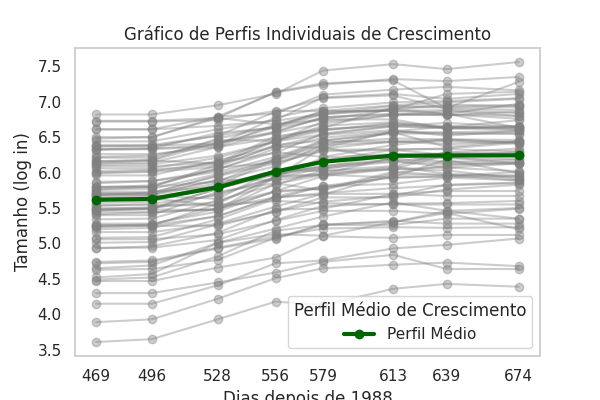
\includegraphics[width=0.7\linewidth]{imagens/secao2/crescimento geral}
	}
	
\end{frame}

\begin{frame}{Análise}
	
	\centering
	\resizebox{\textwidth}{!}{ % 
		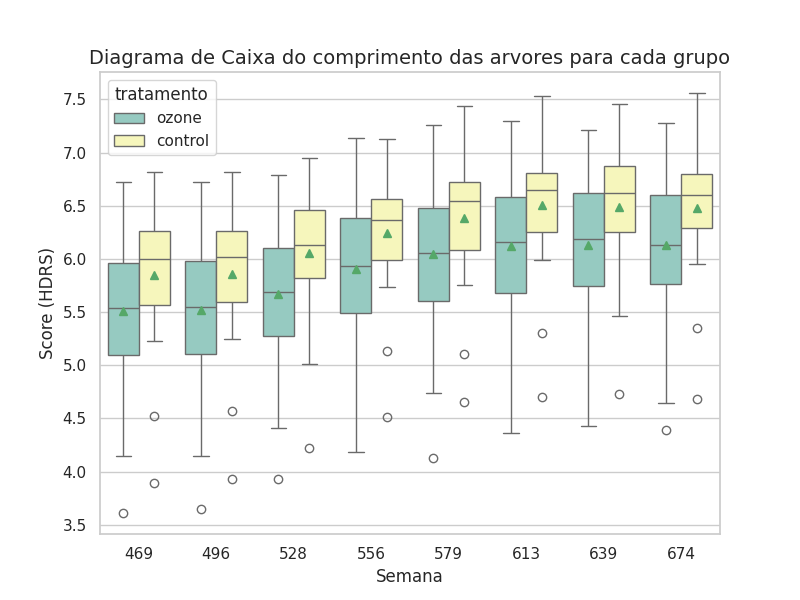
\includegraphics[width=0.7\linewidth]{imagens/secao2/diagrama_de_caixa_crescimento}
	}
	
\end{frame}

\begin{frame}{Análise}
	
	\centering
	\resizebox{\textwidth}{!}{ % 
		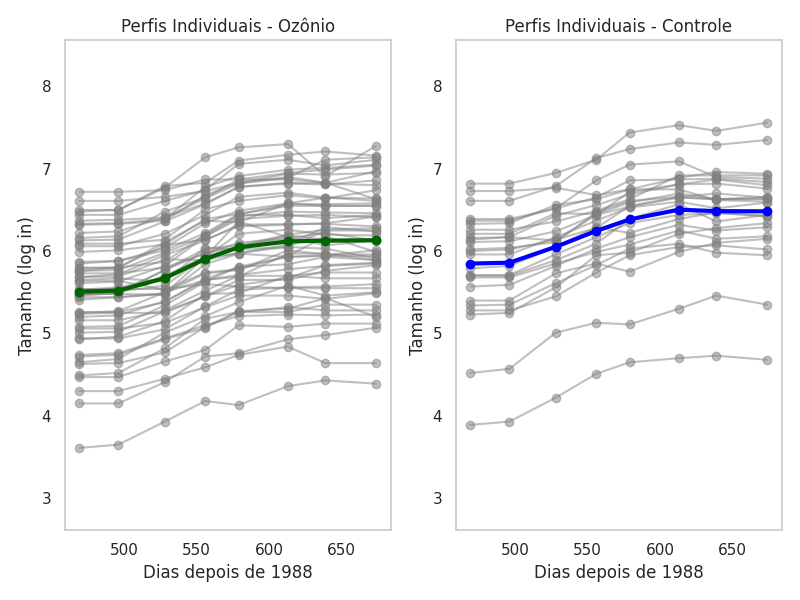
\includegraphics[width=0.7\linewidth]{imagens/secao2/crescimento ozonio e controle}
	}
	
\end{frame}


\begin{frame}{Análise}
	
	\centering
	\resizebox{\textwidth}{!}{ % 
		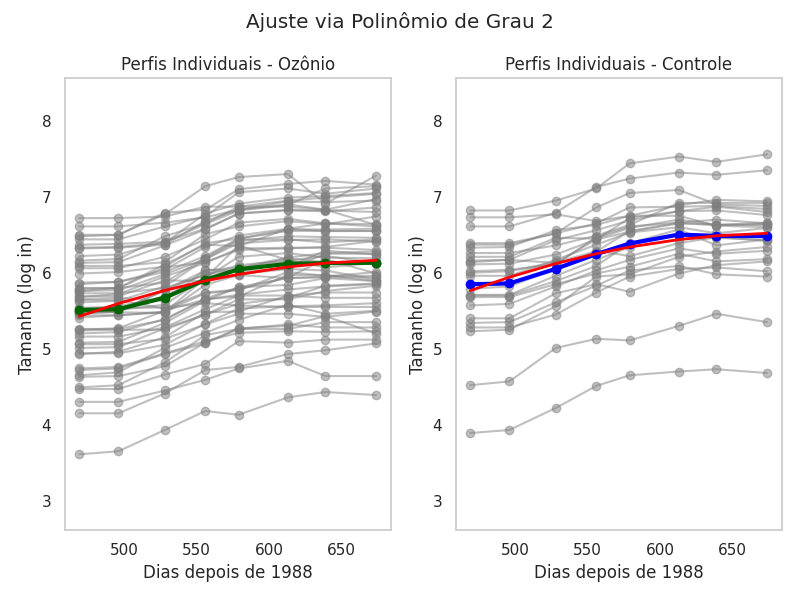
\includegraphics[width=0.7\linewidth]{imagens/secao2/crescimento poli 2}
	}
	
\end{frame}

\begin{frame}{Análise}
	
	\centering
	\resizebox{\textwidth}{!}{ % 
		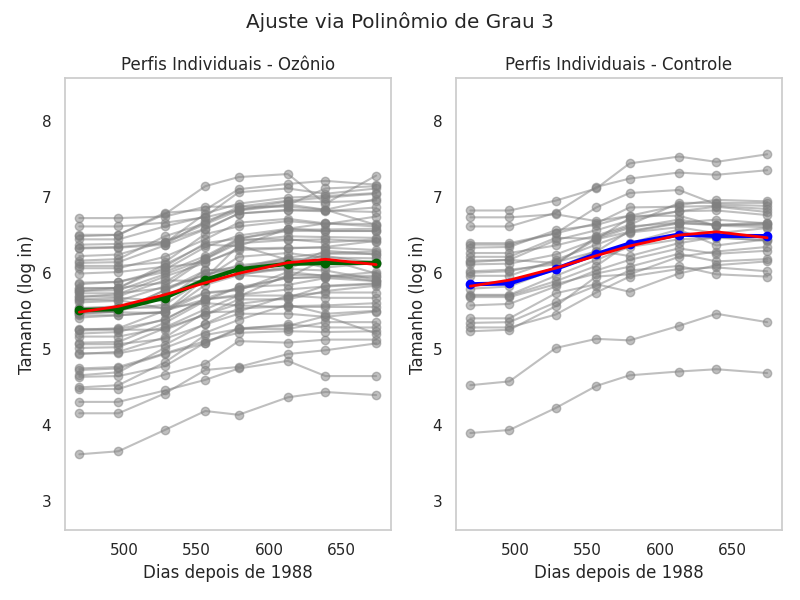
\includegraphics[width=0.7\linewidth]{imagens/secao2/crescimento poli 3}
	}
	
\end{frame}

\begin{frame}{Tentativa de Modelo Misto}
	
	\centering
	\resizebox{\textwidth}{!}{ % 
		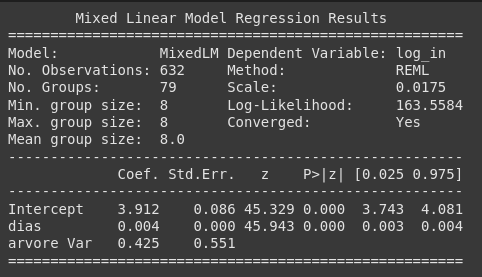
\includegraphics[width=0.7\linewidth]{imagens/secao2/modelo misto}
	}
	
\end{frame}
\begin{frame}{tentativa de Equação de Estimação Generalizada}
	
	\centering
	\resizebox{\textwidth}{!}{ % 
		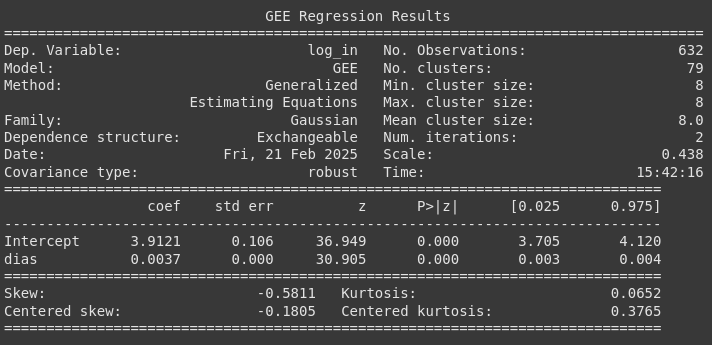
\includegraphics[width=0.7\linewidth]{imagens/secao2/gee}
	}
	
\end{frame}